\documentclass[handout]{beamer}

\usepackage[utf8]{inputenc} % Language and font encoding
\usepackage[icelandic]{babel}
\usepackage[T1]{fontenc}


\usepackage{tikz}
\usepackage[listings,theorems]{tcolorbox}
\usepackage{booktabs}
\usepackage{minted} %Minted and configuration
\usemintedstyle{default}

\renewcommand{\theFancyVerbLine}{\sffamily \arabic{FancyVerbLine}}
%%%%%%%%%%%
% More math
%%%%%%%%%%%
\newcommand{\Mod}[1]{\ \text{mod}\ #1}

%%%%%%%%%%%%%%%%%%%%%%
% Beamer configuration
%%%%%%%%%%%%%%%%%%%%%%
\setbeamertemplate{navigation symbols}{}
\usecolortheme{dove}
\setbeamercolor{frametitle}{fg=white}

\usebackgroundtemplate%
{%
\vbox to \paperheight{

\includegraphics[width=\paperwidth]{Pics/hi-slide-head-2016}

\vfill
\hspace{0.5cm}
\includegraphics[width=0.3\paperwidth]{Pics/hi-von-logo}
\vspace{0.4cm}
    }%
}

\AtBeginSection[]
{
  \begin{frame}<beamer>
    \frametitle{Yfirlit}
    \tableofcontents[currentsection]
  \end{frame}
}

\setbeamerfont{frametitle}{size=\normalsize}
\addtobeamertemplate{frametitle}{}{\vspace*{0.5cm}}

%%%%%%%%%%%%%%%%%%%%%%%%%
% tcolorbox configuration
%%%%%%%%%%%%%%%%%%%%%%%%%

% Setup from: http://tex.stackexchange.com/a/43329/21638
\tcbset{%
    noparskip,
    colback=gray!10, %background color of the box
    colframe=gray!40, %color of frame and title background
    coltext=black, %color of body text
    coltitle=black, %color of title text 
    fonttitle=\bfseries,
    alerted/.style={coltitle=red, colframe=gray!40},
    example/.style={coltitle=black, colframe=green!20, colback=green!5},
}


%%%%%%%%%%%%%%%%%%%%%%%
% Further configuration
%%%%%%%%%%%%%%%%%%%%%%%
\hypersetup{colorlinks=true,pdfauthor={Eirikur Ernir Thorsteinsson},linkcolor=blue,urlcolor=blue}
\graphicspath{{./Pics/}}

\author{Eiríkur Ernir Þorsteinsson}
\institute{Háskóli Íslands}
\date{Haust 2016}

\title{Stærðfræðimynstur í tölvunarfræði}
\subtitle{Vika 7, seinni fyrirlestur}

\begin{document}

\begin{frame}
\titlepage
\end{frame}


\section{Inngangur}

\begin{frame}{Í síðasta tíma}
\begin{itemize}
 \item Talning
 \item Skúffureglan
\end{itemize}
\end{frame}

\section{Umraðanir}

\begin{frame}{Umraðanir og samantektir}
\begin{itemize}
 \item Mörg talningavandamál snúast um fjölda leiða sem við höfum til að velja stök úr mengi
 \begin{itemize}
  \item Stundum skiptir röð stakanna máli
  \item Stundum skiptir hún ekki máli
 \end{itemize}
 \item Setjum fram hugtök til að hjálpa okkur að tala um fjölda slíkra möguleika
\end{itemize}
\end{frame}

\begin{frame}{Umröðun}
\begin{itemize}
 \item Umröðun (e. \emph{permutation}) á mengi er runa sem inniheldur öll stök mengisins
 \item Umröðun $r$ staka úr menginu er kölluð $r$-umröðun (e. \emph{r-permutation}) á menginu
 \item Dæmi: Látum $S = \{1, 2, 3\}$
 \begin{itemize}
  \item Runan $3, 1, 2$ er umröðun á $S$
  \item Runan $3, 2$ er $2$-umröðun á $S$
 \end{itemize}
\end{itemize}
\end{frame}

\begin{frame}{Umraðanir}
Fjöldi $r$-umraðana á mengi með $n$ stök er táknaður með $P(n, r)$.

Til eru lokaðar formúlur fyrir stærðina $P(n,r)$. 

Séu $n$ og $r$ jákvæðar heiltölur, $1 \leq r \leq n$, þá
\[
 P (n, r) = n(n - 1)(n - 2) \ldots (n - r + 1)
\]
séu $n$ og $r$ jákvæðar heiltölur, $0 \leq r \leq n$, þá
\[
 P(n,r) = \frac{n!}{(n-r)!}
\]
\end{frame}

\begin{frame}{Dæmi}
Látum $S = \{a, b, c\}$. $2$-umraðanir $S$ eru $a, b; a, c; b, a;b, c; c, a$ og $c, b$, samtals sex talsins.

Sjáum líka að það eru alltaf sex $2$-umraðanir á 3 staka mengi. Þetta passar við formúlu:
\[
 P(3,2) = \frac{3!}{(3-2)!} = \frac{3!}{(1)!} = \frac{6}{1} = 6
\]
Við hefðum líka getað sannfært okkur um þetta með margfeldisreglu - það eru 3 leiðir til að velja fyrsta stakið og 2 leiðir til að velja það seinna.
\end{frame}

\begin{frame}{Athugun}
Tökum eftir því að það er ein leið til að umraða 0 stökum - þ.e.a.s. ef við höfum engin stök, þá getum við bara myndað tóma runu. Þannig er $P(n,0) = 1$. Þessu ber saman við formúlu:
\[
 P(n,0) = \frac{n!}{(n-0)!} = \frac{n!}{n!} = 1
\]
\end{frame}

\begin{frame}{Athugun}
Tökum líka eftir því að 
\[
 P(n,n) = \frac{n!}{(n-n)!} = \frac{n!}{0!} = n!
\]
sem passar vel við skilning okkar á margfeldisreglu.
\end{frame}

\begin{frame}{Dæmi}
Á hversu marga vegu getum við valið þá sem fá gull, silfur og brons í 100 manna keppni? \pause

Erum að velja þrjá einstaklinga úr 100 staka mengi. Röð einstaklinga skiptir máli. Fáum
\[
 P(100,3) = 100 \cdot 99 \cdot 98 = 970200
\]
\end{frame}

\begin{frame}{Dæmi}
Sölukona þarf að fara til átta mismunandi borga. Fyrsta borgin er föst, en hún má ráða í hvaða röð hún ferðast til hinna borganna. Á hversu marga vegu getur sölukonan valið leið sína, ef hún þarf að fara einu sinni í hverja borg? \pause

Við getum ekki tekið neinar ákvarðanir um fyrstu borgina, en allar mögulegar umraðanir af hinum sjö eru gjaldgengar, svo hún hefur $7! = 5040$ möguleika.

Erfitt vandamál sem tengist þessu: Travelling Salesman Problem.
\end{frame}

\begin{frame}{Dæmi}
Hversu margar af umröðunum stafanna $ABCDEFGH$ innihalda strenginn $ABC$ sem hlutrunu? \pause

Af því að stafirnir $ABC$ þurfa að vera samliggjandi og stafirnir $DEFGH$ eru fimm talsins getum við litið á sem svo að við séum að finna allar mögulegar umraðanir á sex staka mengi. Þá erum við með $6! = 720$ mögulegar umraðanir.
\end{frame}

\section{Samantektir}

\begin{frame}{Samantektir}
\begin{itemize}
 \item Við höfum kynnst umröðunum
 \begin{itemize}
  \item Umröðun á mengi er runa sem inniheldur öll stök mengisins
 \end{itemize}
 \item Skoðum nú samantektir (e. \emph{combinations})
 \begin{itemize}
  \item $r$-samantekt mengis $S$ er $r$ staka hlutmengi í $S$
 \end{itemize}
 \item Samantekt hunsar röð hlutanna
 \begin{itemize}
  \item Þannig ætti ekki að koma á óvart að til séu færri $r$-samantektir fyrir hvert mengi heldur en $r$-umraðanir (þegar $r$ er ekki örsmátt)
 \end{itemize}
 \item Við táknum fjölda $r$-samantekta $n$ staka mengis með $C(n,r)$
\end{itemize}
\end{frame}

\begin{frame}{Dæmi}
Látum $S$ vera mengið $\{a, b, c, d\}$. Þá eru 2-samantektir $S$ sex talsins: $\{a, b\}$, $\{a, c\}$, $\{a, d\}$, $\{b, c\}$, $\{b, d\}$ og $\{c, d\}$. Sem sagt, $C(n, r) = 6$.
\end{frame}

\begin{frame}{Formúla fyrir fjölda samantekta}
Við getum notað deilireglu til að búa til formúlu fyrir fjölda samantekta út frá formúlu fyrir fjölda umraðana ($P(n,r) = \frac{n!}{(n-r)!}$).

Til að finna allar $r$-samantektir getum við fyrst fundið allar $r$-umraðanir og athugað að röðunin skiptir ekki máli. Til eru $P(r,r)$ leiðir til að umraða $r$ stökum, svo hver $r$-samantekt samsvarar $P(r,r)$ mismunandi $r$-umröðunum og deiliregla gefur:
\[
 C(n,r) = \frac{P(n,r)}{P(r,r)} = \frac{n!}{r!(n-r)!}
\]
\end{frame}

\begin{frame}{Dæmi}
Hversu margir bitastrengir af lengd $n$ innihalda nákvæmlega $r$ ása? \pause

Staðsetningar ásanna í bitastrengnum eru $r$-samantekt af menginu $\{1,2,\ldots,n\}$, svo fjöldi bitastrengja af lengd $n$ með nákvæmlega $r$ ása er $C(n, r)$.
\end{frame}

\begin{frame}{Dæmi}
Hversu margar mismunandi 5 spila hendur er hægt að mynda úr 52 spila spilastokk? \pause

Röð spilanna í hverri hönd skiptir ekki máli, svo fjöldinn er
\[
 C(52,5) = \frac{52!}{5!47!} = \frac{52\cdot51\cdot50\cdot49\cdot48}{5!} = 2598960
\]
\pause
En hversu margar 47 spila hendur væri hægt að mynda?
\end{frame}

\begin{frame}{Regla}
Séu $n$ og $r$ ekki-neikvæðar heiltölur, $r \leq n$, þá er
\[
 C(n,r) = C(n,n-r)
\]
Þetta má sjá með innsetningu í formúluna 
\[
 C(n,r) = \frac{n!}{r!(n-r)!}
\]
\end{frame}

\begin{frame}{Talningarsannanir}
\begin{itemize}
 \item Hægt er að rökstyðja $C(n,r) = C(n,n-r)$ með bókstafareikningi
 \item Svona jöfnur mætti líka rökstyðja með talningu:
 \begin{itemize}
  \item Sönnun með tvöfaldri talningu (e. \emph{double counting proof}): Notum talningu til að sýna að báðar hliðar jöfnu gefi sama fjölda
  \item Sönnun með gagntæku falli (e. \emph{bijective proof}): Sýnum að til sé gagntækt fall milli þeirra hluta sem taldir eru öðru megin jöfnu og þeirra hluta sem taldir eru á hinni hliðinni
 \end{itemize}
\end{itemize}
\end{frame}

\section{Tvíliður}

\begin{frame}{Tvíliður}
\begin{itemize}
 \item $C(n,k)$ er oft táknað með $\binom{n}{k}$, þá kallað tvíliðustuðull (e. \emph{binomial coefficient})
 \item Tvíliða (e. \emph{binomial expression}) er summa tveggja liða, t.d. $x + y$
 \item Tvíliðustuðlar koma fram þegar tvíliða er hafin í veldi
 \begin{itemize}
  \item Stuðullinn við $x^ry^{n-k}$ er $C(n,k) = \binom{n}{k}$ þegar $(x + y)^n$ er reiknað út
 \end{itemize}
\end{itemize}
\end{frame}

\begin{frame}{Dæmi}
Reglan: Stuðullinn við $x^ry^{n-k}$ er $C(n,k) = \binom{n}{k}$ þegar $(x + y)^n$ er reiknað út

Fáum:
\begin{align*}
(x+y)^3 &= \binom{3}{0} x^3 + \binom{3}{1}x^2y + \binom{3}{2}xy^2 + \binom{3}{3}y^3\\
&= x^3 + 3x^2y + 3xy^2 + y^3
\end{align*}

\end{frame}

\begin{frame}{Talning á stuðlum}
\begin{itemize}
 \item Við getum sannfærst um að $(x+y)^3 = x^3 + 3x^2y + 3xy^2 + y^3$ með því að nota talningu í stað þess að nota bókstafareikning.
 \item Við myndum liði sem innihalda $x^3$, $x^2y$, $xy^2$ og $y^3$ með því að ``velja'' $x$ og $y$ úr $(x+y)(x+y)(x+y)$.
 \begin{itemize}
  \item Til að mynda lið sem inniheldur $x^3$ þarf að velja $x$ úr öllum svigunum, einungis ein leið er til að gera það svo $x^3$ er með stuðulinn 1. 
  \item Til að mynda lið sem inniheldur $x^2y$ þarf að velja $x$ í tveimur af þremur svigum, sem er hægt að gera á $C(3,2) = \binom{3}{2}$ vegu, o.s.frv.
 \end{itemize}
\end{itemize}
\end{frame}

\begin{frame}{Tvíliðusetningin}
\begin{tcolorbox}[title=Tvíliðusetningin]
Látum $x$ og $y$ vera liði og $n$ vera ekki-neikvæða heiltölu. Þá
\[
 (x + y)^n = \sum_{r=0}^n \binom{n}{r} n^{n-r} y^r
\]
\end{tcolorbox}
\end{frame}

\begin{frame}{Fylgisetning}
\begin{tcolorbox}[title=Fylgisetning tvíliðusetningarinnar]
Látum $n$ vera ekki-neikvæða heiltölu. Þá
\[
 \sum_{k=0}^n \binom{n}{k} = 2^n
\]
\end{tcolorbox}
Getum rökstutt þetta með talningu. $2^n$ er fjöldi hlutmengja $n$ staka mengis, hvert hlutmengjanna er með fjölda staka á bilinu $0$ upp í $n$ (bæði með talin). Fjöldi 0 staka hlutmengja er $\binom{n}{0}$, fjöldi 1 staks hlutmengja er $\binom{n}{1}$\ldots
\end{frame}

\begin{frame}{Jafna Pascals}
Tvíliðustuðlar uppfylla margar jöfnur, sú frægasta er jafna Pascals (1623-1662):
\[
\binom{n+1}{k} = \binom{n}{k-1} + \binom{n}{k}
\]
þar sem $n$ og $k$ eru jákvæðar heiltölur, $n \geq k$. Þetta má rökstyðja með bókstafareikningi eða talningu.
\end{frame}

\begin{frame}{Þríhyrningur Pascals}
\begin{center}
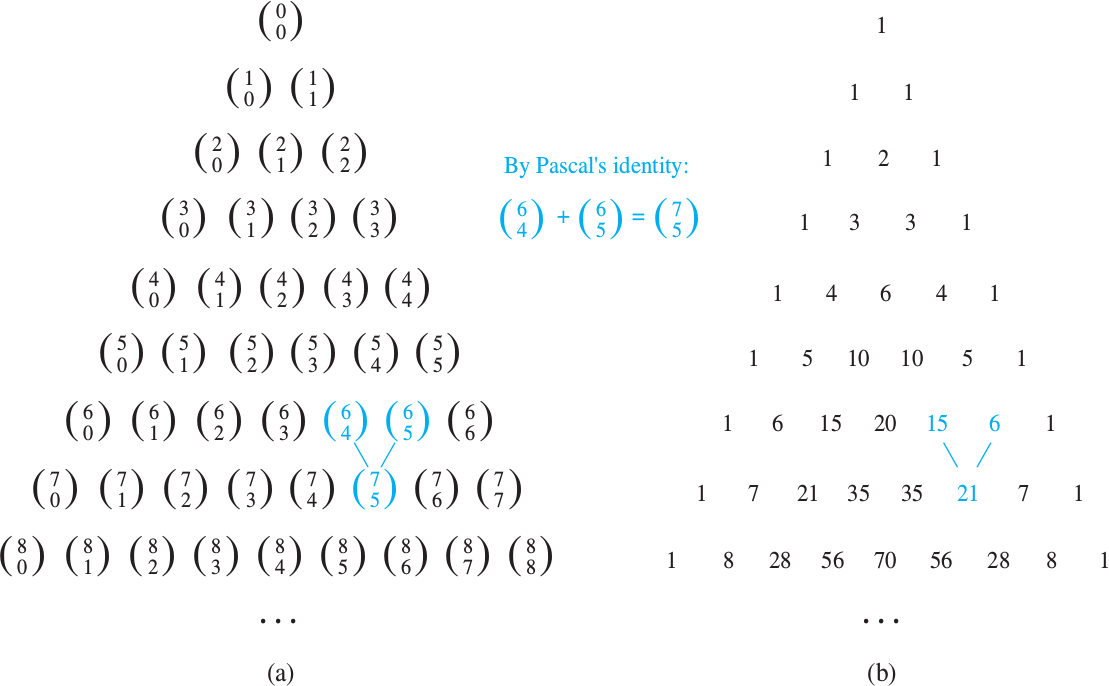
\includegraphics[width=\textwidth]{pascal}
\end{center}
\end{frame}

\begin{frame}{Þríhyrningur Yanghuis}
\begin{columns}
\column{0.3\textwidth}
Þríhyrningur Yanghuis, frá 1303.
\column{0.7\textwidth}
\begin{center}
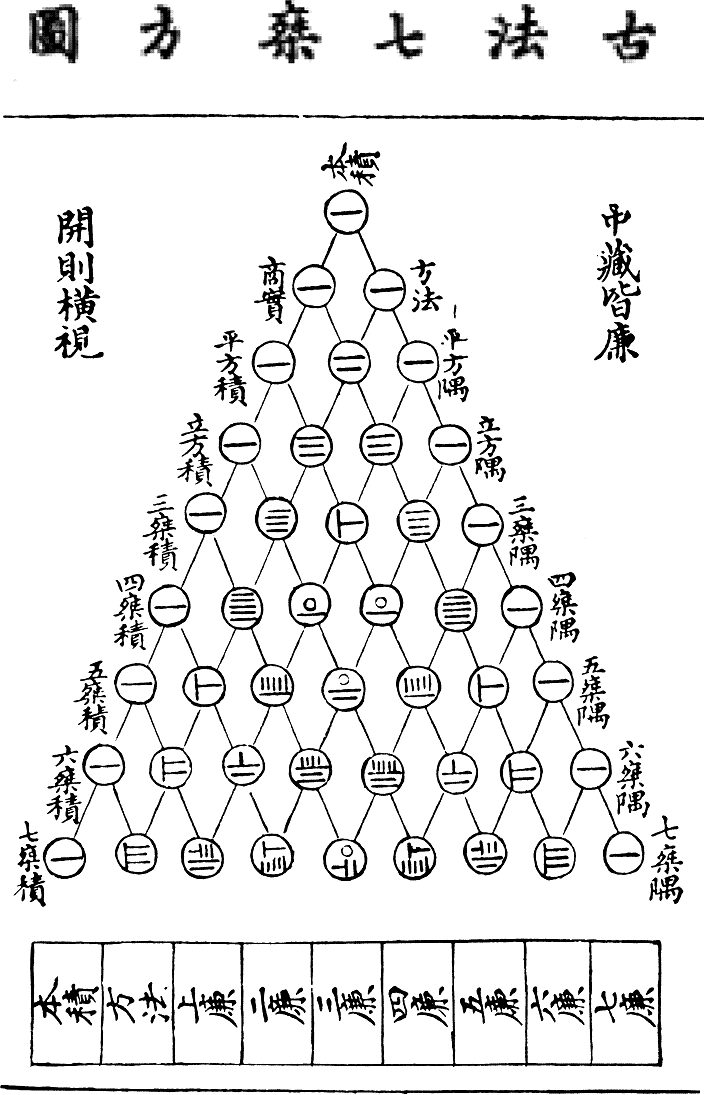
\includegraphics[width=0.5\linewidth]{yanghui}
\end{center}
\end{columns}
\end{frame}

\begin{frame}{Sierpinski þríhyrningurinn}
\begin{columns}
\column{0.3\textwidth}
Séu oddatölurnar í Pascal-þríhyrningnum litaðar fæst mynstur líkt fraktanum sem kallaður er þríhyrningur Sierpinskis.
\column{0.7\textwidth}
\begin{center}
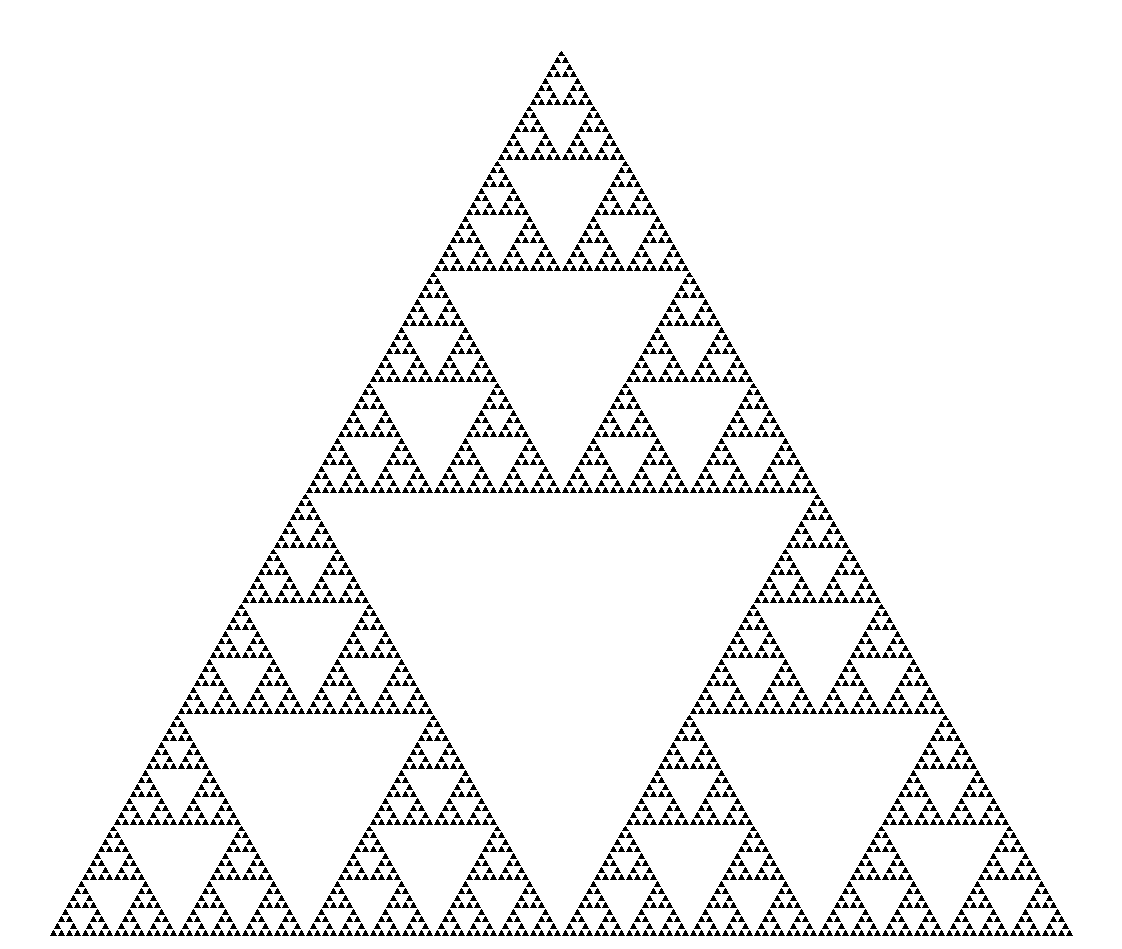
\includegraphics[width=\linewidth]{sierpinski}
\end{center}

\end{columns}

\end{frame}

\begin{frame}{Þríhyrningur Pascals}
\begin{center}
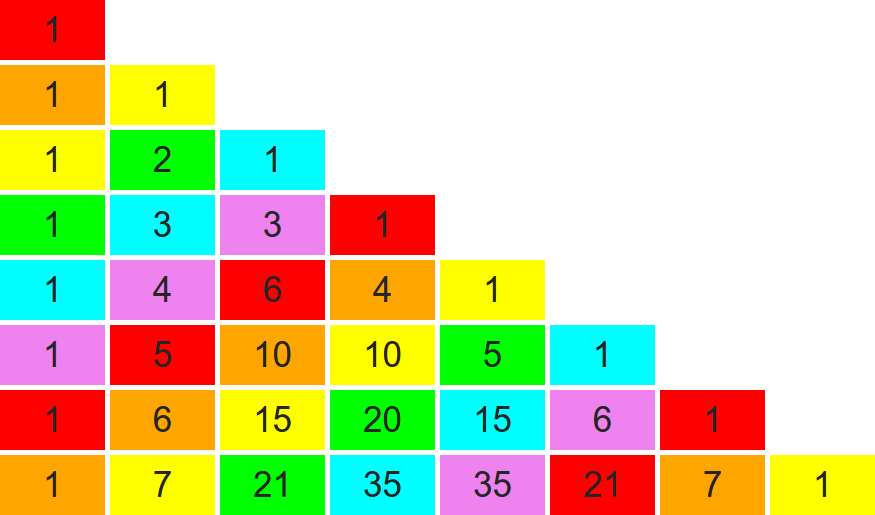
\includegraphics[width=\textwidth]{pascal-bands}
\end{center}
\end{frame}

\begin{frame}{Næst}
Talning fyrir lengra komna. Kaflar 8.1, 8.2, mögulega 8.3.
\end{frame}

\end{document}
